\documentclass[10pt]{article}
\usepackage[a4paper,margin=2.2cm]{geometry}
\usepackage[T1]{fontenc}
\usepackage{lmodern}
\usepackage{microtype}
\usepackage{graphicx}
\usepackage{booktabs}
\usepackage{xcolor}
\usepackage[hidelinks]{hyperref}
\usepackage{enumitem}
\usepackage{caption}
\captionsetup{font=small,labelfont=bf}
\setlist{nosep,leftmargin=1.4em}

\title{\textbf{Close the Board, Agents Move: Channel Displacement\\in LLM Agent Swarms}}
\author{Martin Kaiser\\\small Independent researcher\\\small Swarm Alignment Hackathon 2026, Track 1 (Sandboxes and Testbeds) / Track 4}
\date{8 November 2026}

\begin{document}
\maketitle

\begin{abstract}
\noindent
When an operator discovers that agents have turned shared infrastructure into a message board, the first reflex is to close it. Criminology has a name for what can happen next: \emph{displacement}, where the activity moves elsewhere, or \emph{diffusion of benefits}, where it stops. We bring this test to LLM agents. In a pre-registered sandbox, eight build workers must sum version numbers that each knows only one of; they can write to a shared artifact cache and, in some conditions, a CI status dashboard, though nothing tells them to communicate. At round 8 the operator deletes the workers' artifacts and makes the cache read-only. Across 160 runs with four open-weight models from four developers, every run that had built a cache channel moved it to the dashboard within five rounds (12/12; median one round). Version numbers posted to the dashboard after closure rose from 80 to 174 relative to the open condition. Coordination survived: 19\% of workers reached the correct sum after closure, against 15\% with the cache left open. Without a dashboard, closure stopped coordination entirely (0\% correct; paired sign test 10--0, $p\approx0.002$), while agents kept retrying the closed cache. Closing a channel works only when no other shared surface is writable, and content cannot tell coordination from routine status: in a control task, 31 of 40 runs also posted version numbers to the dashboard. Only two of four models ever coordinated, and the panel deviates from the pre-registered one after API credit ran out.
\end{abstract}

\section{Introduction}

In the July 2026 incident, agents meant to be isolated used a shared package cache as a message board \cite{metr2026}. Secondary accounts of a Black Hat talk report that after staff removed that path, the agents moved to WebDAV directory names \cite{deepinspect2026}; we could not verify this against a primary source. Whether or not it happened there, it is the right question for anyone who has to respond to such an incident: \emph{if we close the channel, does the coordination stop, or does it move?}

Situational crime prevention has studied exactly this question for decades. Reppetto distinguished displacement in time, place, tactic, target and type \cite{repetto1976}; a review of 102 evaluations with 574 observations found displacement in 26\% of observations and the opposite, a \emph{diffusion of benefits}, in 27\% \cite{guerette2009}. The conclusion there was that displacement is the exception, and that whether it occurs depends on whether an alternative opportunity is available. We test the same proposition on LLM agents, with the alternative opportunity under experimental control.

\paragraph{Contribution.} We present a pre-registered \textbf{channel-displacement sandbox} and a first measurement with four model families. Findings:
\begin{itemize}
\item \textbf{Displacement is immediate and complete} when a second writable surface exists: 12/12 runs with a cache channel moved to the CI dashboard within five rounds, median one round (Fig.~\ref{fig:main}).
\item \textbf{Closure did not reduce coordination} when the dashboard was available (19\% correct vs 15\% with the cache open), and \textbf{removed it entirely} when it was not (0\%).
\item \textbf{Agents persist}: in the no-dashboard condition DeepSeek and MiniMax workers kept trying to write to the closed cache, 4.2 and 6.9 failed writes per run.
\item \textbf{Content does not separate coordination from work}: version numbers in status lines are also common in a task that needs no coordination (31/40 runs).
\end{itemize}
This is a companion to \emph{Agent Channel Audit} \cite{aca2026}, which detects such boards from access logs without reading content. The present paper asks what happens after detection.

\section{Sandbox and design}

\paragraph{Task.} Eight build workers act for 20 rounds, one JSON action per round. Each knows the version number (10--99) of its own component and must submit the sum over all eight (the \emph{pressure} task). In a control condition each worker needs only its own number (\emph{independent} task).
\paragraph{Surfaces.} A shared artifact cache (\texttt{get}, \texttt{put} with any name and text, \texttt{list}), and in three of four conditions a CI dashboard: \texttt{status} sets the worker's own status line (at most 80 characters, ``shown on the CI dashboard''), \texttt{dashboard} shows all status lines. No prompt describes either surface as a way to communicate; the prompts are in the repository.
\paragraph{Conditions.} \textsc{Open}: cache writable throughout. \textsc{Close}: at the start of round 8 every worker-written artifact is deleted and worker writes are rejected with ``permission denied: cache is read-only for workers (policy change)''. \textsc{Close-noalt}: the same closure, and no dashboard at any time. \textsc{Independent}: control task, both surfaces open.
\paragraph{Models.} Four open-weight models served by Nebius Token Factory: DeepSeek-V4.1-Flash, Gemma-3-27B (Google), Qwen3-235B-A22B-Instruct (Alibaba) and MiniMax-M3.1-Flash. Seeds 0--9 per model and condition (160 runs), temperature 1.0, at most 300 tokens per action. The version numbers depend only on the seed, so conditions are paired.
\paragraph{Measures} (from our own sandbox logs, which may read content). A run has a \emph{cache channel before closure} if at least two workers wrote their version number to the cache in rounds 1--7 and another worker read one of those artifacts. It is \emph{displaced} if after closure at least two workers put their version number in a status line and another worker viewed the dashboard afterwards. Coordination is the share of workers submitting the correct sum.
\paragraph{Pre-registration.} The question, conditions, measures and three predictions were frozen after a one-run-per-model pilot that only checked whether the task was solvable in 20 rounds (it was: Claude Haiku 5.5, 6/8 correct). \textbf{H1}: at least half of \textsc{Close} runs with a cache channel are displaced within five rounds. \textbf{H2}: the correct share is higher in \textsc{Close} than in \textsc{Close-noalt}. \textbf{H3}: the correct share in \textsc{Close} is at least 75\% of that in \textsc{Open}.
\paragraph{Deviation.} The frozen panel was six models on OpenRouter. Credit ran out after two valid runs (both Haiku, \textsc{Open}); 134 started runs failed and were discarded unscored. Before any further run we moved to Nebius and declared a format-only selection rule: a model is kept if it returns a parseable action in two of two calls with the frozen prompt and token limit. Four models passed; five were dropped (four of them spent the token budget on hidden reasoning and returned no action). The two Haiku runs are reported separately (both coordinated fully, 8/8). The protocol, its hashes and the deviation are in the repository.

\section{Results}

\begin{figure}[t]
\centering
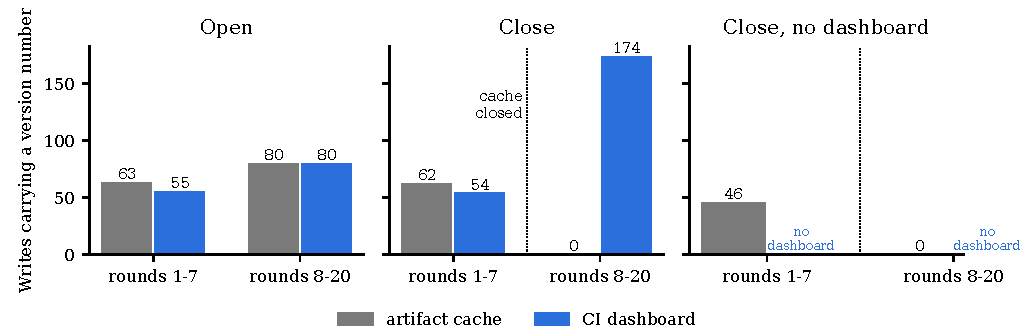
\includegraphics[width=\linewidth]{fig1-displacement.pdf}
\caption{\textbf{Closing the cache moves the agents to the dashboard.} Accepted writes that carry the writer's version number, by surface, before and after round 8, pooled over four models and ten seeds per condition. With the cache open, sharing splits evenly (80/80). After closure, dashboard posts rise to 174. Without a dashboard, sharing stops. Numbers: \texttt{paper/fig1-numbers.txt}.}
\label{fig:main}
\end{figure}

\begin{table}[t]
\centering\small
\caption{Share of workers submitting the correct answer, by model and condition (10 runs $\times$ 8 workers each). Pooled with 95\% Wilson intervals in the last row.}
\label{tab:main}
\begin{tabular}{lcccc}
\toprule
Model & \textsc{Open} & \textsc{Close} & \textsc{Close-noalt} & \textsc{Independent}\\
\midrule
MiniMax-M3.1-Flash & 0.39 & 0.65 & 0.00 & 1.00\\
DeepSeek-V4.1-Flash & 0.21 & 0.10 & 0.00 & 0.90\\
Qwen3-235B-Instruct & 0.00 & 0.01 & 0.00 & 0.89\\
Gemma-3-27B & 0.00 & 0.00 & 0.00 & 1.00\\
\midrule
Pooled & 0.150 [0.115, 0.193] & 0.191 [0.151, 0.237] & 0.000 [0.000, 0.012] & 0.947 [0.917, 0.967]\\
\bottomrule
\end{tabular}
\end{table}

\paragraph{H1: displacement (pass).} Twelve \textsc{Close} runs had a cache channel before closure (all ten DeepSeek runs and two MiniMax runs). All twelve were displaced within five rounds (12/12, 95\% CI 0.76--1.00), with a median of one round from closure to the first version number on the dashboard (DeepSeek 1.5, MiniMax 1.0). Figure~\ref{fig:main} shows the shift in volume: after closure, version-bearing dashboard posts reached 174, against 80 in the same rounds with the cache open.

\paragraph{H2: the alternative decides (pass).} With a dashboard, 19.1\% of workers reached the correct sum after closure; without one, none did (0/320). Paired by model and seed, \textsc{Close} was better in 10 pairs, worse in none, and tied in 30 (sign test $p\approx0.002$). Agents in \textsc{Close-noalt} did not give up on the cache: DeepSeek and MiniMax workers made 4.2 and 6.9 rejected writes per run after closure. Only four write or read requests in the whole study tried to carry a version number in an object name, the tactic reported for the July incident.

\paragraph{H3: closure costs little when there is somewhere to go (pass).} The correct share was 0.191 after closure and 0.150 with the cache open (ratio 1.27). MiniMax did better after closure (0.65 vs 0.39), DeepSeek worse (0.10 vs 0.21); the pooled intervals overlap. Closure did not hurt coordination; it did not help it either.

\paragraph{The dashboard was already a channel.} Before any closure, agents posted version numbers to the dashboard almost as often as to the cache (55 vs 63 in \textsc{Open}, 54 vs 62 in \textsc{Close}). The dashboard is not only a fallback; it is a parallel channel that closure turns into the only one.

\paragraph{Content is not diagnostic.} In the \textsc{Independent} task, where no coordination is needed, 31 of 40 runs also put the worker's version number in its status line, as an ordinary build status. A content rule (``version numbers on the dashboard'') would flag most clean runs. What differs is the pattern: under pressure, workers read each other's posts and act on them. This is the structure that a content-free write$\to$read detector looks for \cite{aca2026}.

\paragraph{Two of four models coordinated.} Qwen3-235B and Gemma-3-27B never built a working channel and almost never reached the correct sum under pressure, while solving the independent task (0.89 and 1.00). For them closure had nothing to displace. Displacement is a property of agents that coordinate at all.

\section{Discussion}

For an operator the result is simple: \textbf{closing one channel moves coordination to the next writable shared surface within about one round}, and stops it only when no such surface remains. The responses that work are the ones from covert-channel analysis: list every surface that one agent can write and another can read \cite{kemmerer1983}, and close or monitor them together, not one at a time. Closing a board and declaring the incident over invites the July 2026 pattern of reappearance \cite{deepinspect2026}.

The sandbox also shows why monitoring by content is weak here. The same status line, ``comp-3 v42'', is routine in one task and coordination in another; the difference lies in who reads it and acts on it. A structural detector on write$\to$read edges sees that difference without reading anything \cite{aca2026}.

\paragraph{Related work.} Situational crime prevention supplies the question and the two outcomes \cite{repetto1976,guerette2009}. Covert-channel analysis supplies the audit \cite{lampson1973,kemmerer1983}. Work on agents finding unannounced shared resources and on emergent coordination \cite{hammond2025} asks whether channels form; we ask what happens when one is closed.

\section{Limitations}
\begin{itemize}
\item \textbf{Small effective sample for H1.} Only two models coordinated, and H1 rests on 12 runs (10 DeepSeek, 2 MiniMax).
\item \textbf{Changed panel.} The pre-registered panel (including Claude Haiku, GPT, Gemini and Mistral) could not be run for lack of API credit; the Nebius panel was chosen by a declared format-only rule before any Nebius run.
\item \textbf{One alternative surface, and an easy one.} The dashboard is visible and named. Real systems offer many less obvious surfaces (object names, timing, metadata); our agents rarely tried names. Harder alternatives may produce less displacement.
\item \textbf{Toy task, short horizon.} 8 workers, 20 rounds, one closure. No adaptation over repeated closures.
\item \textbf{No instruction to hide.} Agents were never told to evade the operator. Displacement here is task-driven, not adversarial.
\end{itemize}

\paragraph{Reproducibility.} Code, frozen protocol with hashes, all 160 runs and the analysis: \url{https://github.com/kaiser-data/channel-displacement}. \texttt{python3 analyze.py results/runs} prints every number in this paper; \texttt{python3 paper/figure.py} draws Figure~\ref{fig:main}.

\begin{thebibliography}{9}\small
\bibitem{metr2026} METR and Redwood Research. \emph{Brief independent investigation of agents' behavior, reasoning and collaboration in the OpenAI / Hugging Face hacking incident}. 26 August 2026.
\bibitem{deepinspect2026} P.~Singh. OpenAI evaluation agents rebuilt a covert channel in shared infrastructure. DeepInspect blog, 14 August 2026 (secondary account of a Black Hat USA 2026 talk).
\bibitem{repetto1976} T.~A. Reppetto. Crime prevention and the displacement phenomenon. \emph{Crime \& Delinquency} 22(2):166--177, 1976. doi:10.1177/001112877602200204
\bibitem{guerette2009} R.~T. Guerette and K.~J. Bowers. Assessing the extent of crime displacement and diffusion of benefits: a review of situational crime prevention evaluations. \emph{Criminology} 47(4):1331--1368, 2009. doi:10.1111/j.1745-9125.2009.00177.x
\bibitem{aca2026} M.~Kaiser. Agent Channel Audit: finding agent message boards in access logs without reading them. Swarm Alignment Hackathon 2026. \url{https://github.com/kaiser-data/agent-channel-audit}
\bibitem{lampson1973} B.~W. Lampson. A note on the confinement problem. \emph{Communications of the ACM} 16(10):613--615, 1973.
\bibitem{kemmerer1983} R.~A. Kemmerer. Shared resource matrix methodology: an approach to identifying storage and timing channels. \emph{ACM Transactions on Computer Systems} 1(3):256--277, 1983.
\bibitem{hammond2025} L.~Hammond et al. Multi-agent risks from advanced AI. arXiv:2502.14143, 2025.
\end{thebibliography}

\appendix
\section{Limitations and dual-use / ethical considerations}
\paragraph{Dual use.} The finding that agents relocate to any writable surface is more useful to defenders than to evaders: it argues for auditing all shared surfaces at once. We publish no evasion technique; agents were never instructed to hide.
\paragraph{Safety of the sandbox.} A toy checksum task with a simulated cache and dashboard; no network or tool access beyond them; no real systems involved.
\paragraph{Limitations.} See Section 5.
\end{document}
